\documentclass{article}

\usepackage[english]{babel}


\usepackage[a4paper,top=2cm,bottom=2cm,left=3cm,right=3cm,marginparwidth=1.75cm]{geometry}

\usepackage{pgfplots}
\pgfplotsset{width=15cm,height=12cm,compat=1.16}
\usepackage{amsmath}
\usepackage{xcolor}
\usepackage{graphicx}
\usepackage{listings}
\usepackage[colorlinks=true, allcolors=blue]{hyperref}
\definecolor{light-gray}{gray}{0.95}

\pgfplotsset{compat=1.18}
\title{COL216 Assignment 3}
\author{Dhruv Gupta 2021CS50125 \\ Niranjan Sarode 2021CS50612}
\date{}
\begin{document}
\maketitle

\section{Introduction}

\subsection{Problem Statement}
\begin{itemize}
    \item In this Assignment we were required to implement a cache simulator with 2 level caches L1 and L2 in C++ which reads a trace file and counts the hits,misses,reads,writes etc for both the caches and prints the stats.
    \item \verb|w	400341a0|  This is a write (read if start in r) operation at address 400341a0 (hexadecimal address).
    \item Cache eviction policy: Simulator uses least replacement policy (LRU).
    \item Cache write policy: Simulator uses Write-back Write-allocate (WBWA).
\end{itemize}

\subsection{Design Decisions}

\begin{itemize}
    \item We have used a struct to represent a cache line. It has the following fields:
    \begin{itemize}
        \item Valid 
        \item Dirty 
        \item Tag 
        \item Value
    \end{itemize}
    \item for LRU we used a vector of size equal to the associativity of the cache. Each element of the vector represents a cache line. The element at index i represents the ith most recently used cache line. 
    \item For a read Instruction (identified by r) 
    \begin{itemize}
        \item We find index bits tag bits  and offset bits for both L1 and L2 from the address
        \item Then we check L1 cache from the L1 index bits
        \item If its tag matches with cache block tag, its valid is true then its a read-L1-hit.
        \item Otherwise (if its invalid or tag doesn't match) then its a read-L1-miss then it searches in L2
        \item Writeback the least used element in LRU to L2 if its dirty bit is true
        \item Then we check in L2 cache from the L2 index bits
        \item If its tag matches with cache block tag, its valid is true then its a read-L2-hit then replaces the least recently used block in L1. 
        \item Otherwise (if its invalid or tag doesn't match) then its a read-L2-miss then it \textcolor{blue}{searches in memory} and replaces the least recently used block in L2  and it  replaces the least recently used block in L1. 
    \end{itemize}
    \item For a write Instruction (identified by w)
    \begin{itemize}
        \item We find index bits tag bits  and offset bits for both L1 and L2 from the address
        \item Then we check L1 cache from the L1 index bits
        \item If its tag matches with cache block tag, its valid is true then its a write-L1-hit then we Modify the dirty attribute to true for that block.
        \item Otherwise (if its invalid or tag doesn't match) then its a write-L1-miss.
        \item Writeback the least used element in LRU to L2 if its dirty bit is true
        \item Then we check in L2 cache from the L2 index bits
        \item If its tag matches with cache block tag, its valid is true then its a read-L2-hit.Modify the dirty attribute to true for that block and replace the least recently used block in L1. 
        \item Otherwise (if its invalid or tag doesn't match) then its a read-L2-miss then it \textcolor{blue}{searches in memory} and replaces the least recently used block in L2 replaces the least recently used block in L1. 
    \end{itemize}
    \item For writeback to L2 from L1:
    \begin{itemize}
        \item We find index bits tag bits  and offset bits for L2.
        \item Check if block is found in L1 if yes then write in L2 and make dirty bit true.
        \item Otherwise (if its invalid or tag doesn't match) then its a write-L2-miss and \textcolor{blue}{value is read from memory and written in L2.}
    \end{itemize}
\end{itemize}


\newpage
\section{Results and Analysis}

\subsection{Graphs}


\subsubsection{Variation in Block Size}
Graph obtained by varying block size on x-axis between 8, 16, 32, 64, 128, and keeping L1 size,
L1 associativity, L2 size and L2 associativity fixed at 1024, 2, 65536, 8 :-


\begin{figure}[h]
    \centering
    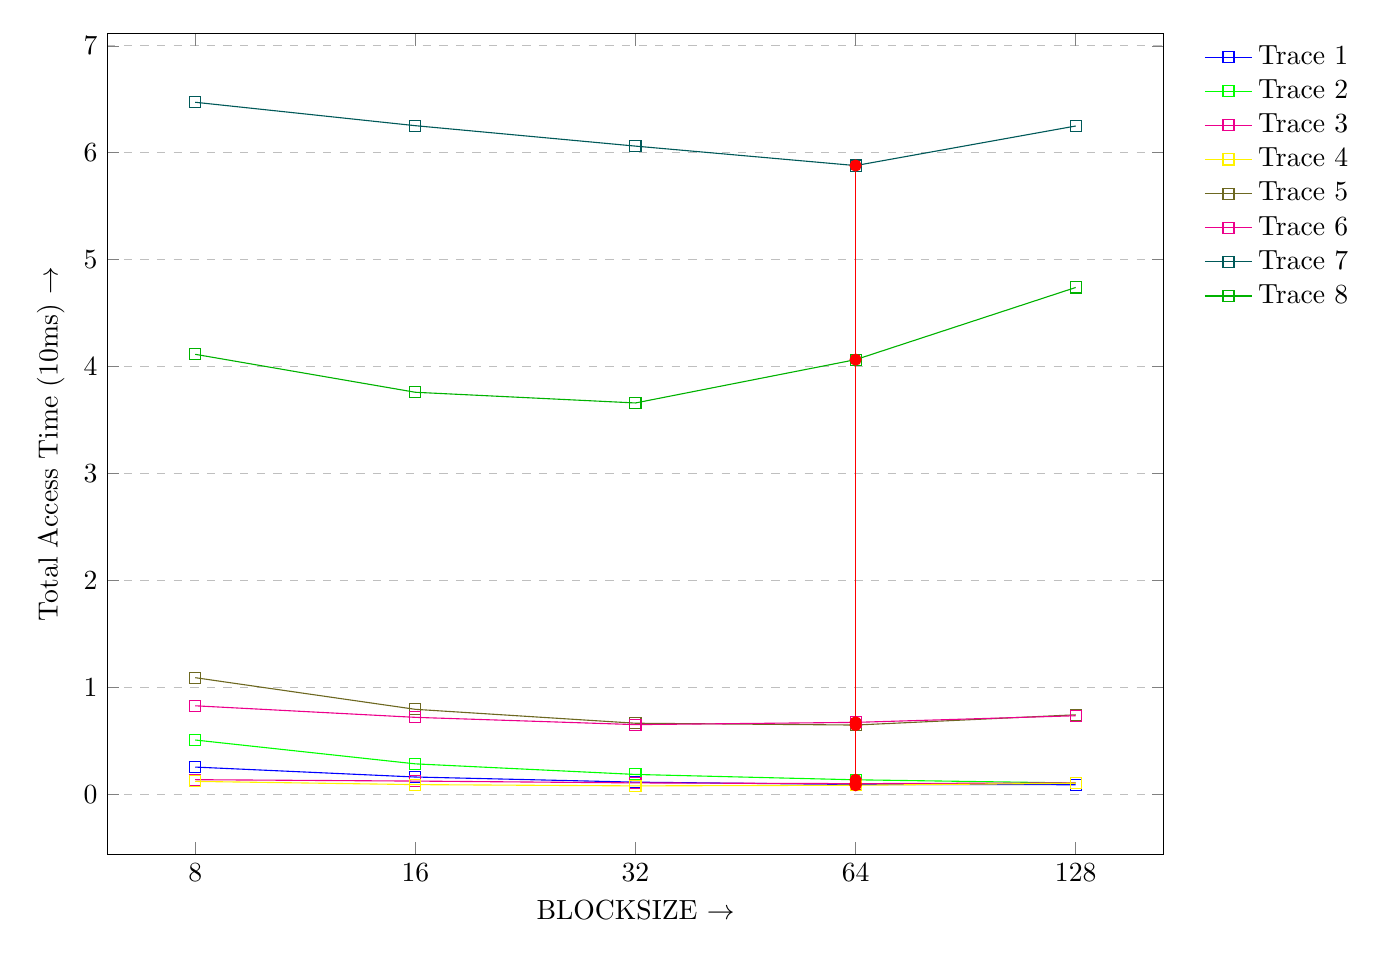
\begin{tikzpicture}
    \begin{axis}[
        xlabel={BLOCKSIZE $\rightarrow$},
        ylabel={Total Access Time (10ms) $\rightarrow$},
        xtick=data,
        symbolic x coords={8,16,32,64,128},
        legend pos=outer north east,
        legend style={draw=none},
        ymajorgrids=true,
        grid style=dashed,
    ]
    \addplot[color=blue,mark=square] coordinates {
        (8,0.255) (16,0.162) (32,0.114) (64,0.092) (128,0.09)};
    \addplot[color=green,mark=square] coordinates {
        (8,0.508) (16,0.285) (32,0.186) (64,0.136) (128,0.106)};
    \addplot[color=magenta,mark=square] coordinates {
        (8,0.137) (16,0.124) (32,0.107) (64,0.1) (128,0.107)};
    \addplot[color=yellow,mark=square] coordinates {
        (8,0.121) (16,0.091) (32,0.079) (64,0.085) (128,0.104)};
    \addplot[color=olive!70!black,mark=square] coordinates {
        (8,1.091) (16,0.795) (32,0.665) (64,0.648) (128,0.744)};
    \addplot[color=magenta,mark=square] coordinates {
        (8,0.828) (16,0.72) (32,0.652) (64,0.673) (128,0.735)};
    \addplot[color=teal!70!black,mark=square] coordinates {
        (8,6.472) (16,6.253) (32,6.062) (64,5.88) (128,6.25)};
    \addplot[color=green!70!black,mark=square] coordinates {
        (8,4.115) (16,3.76) (32,3.66) (64,4.065) (128,4.74)};
    \addplot[color=red,mark=*] coordinates {
        (64,0.092) (64,0.136) (64,0.1) (64,0.085) (64,0.648) (64,0.673) (64,5.88) (64,4.065)};
    \legend{Trace 1,Trace 2,Trace 3,Trace 4,Trace 5,Trace 6,Trace 7,Trace 8,}
    \end{axis}
    \end{tikzpicture}
    \caption{Variation in blocksize}\label{fig:BS}
    \end{figure}

\begin{itemize}
    \item \textbf{Theoretical Expectation} : As the block size increases, the number of blocks that can fit in a cache line increases, which \textcolor{blue}{reduces the number of cache misses}. Therefore, we expect to see a decrease in the miss rate and total access time as the block size increases. However, as the block size becomes larger, the \textcolor{red}{cache line may become less efficient due to unused data}. Hence, there is an optimal block size that minimizes the miss rate and access time.
    \item We see that total access time decreases then increases which matches with the theoretical expectation. The variation is significant for trace 7 and trace 8. The default value of 64 is high enough to give a decent performance for some of  the traces. 
\end{itemize}


\newpage
\subsection{Variation in L1 size}
In the second graph, vary the second parameter L1 size between 512, 1024, 2048,
4096, 8192, and keep block size, L1 associativity, L2 size and L2 associativity fixed at
64, 2, 65536, 8.
\begin{figure}[h]
    \centering
    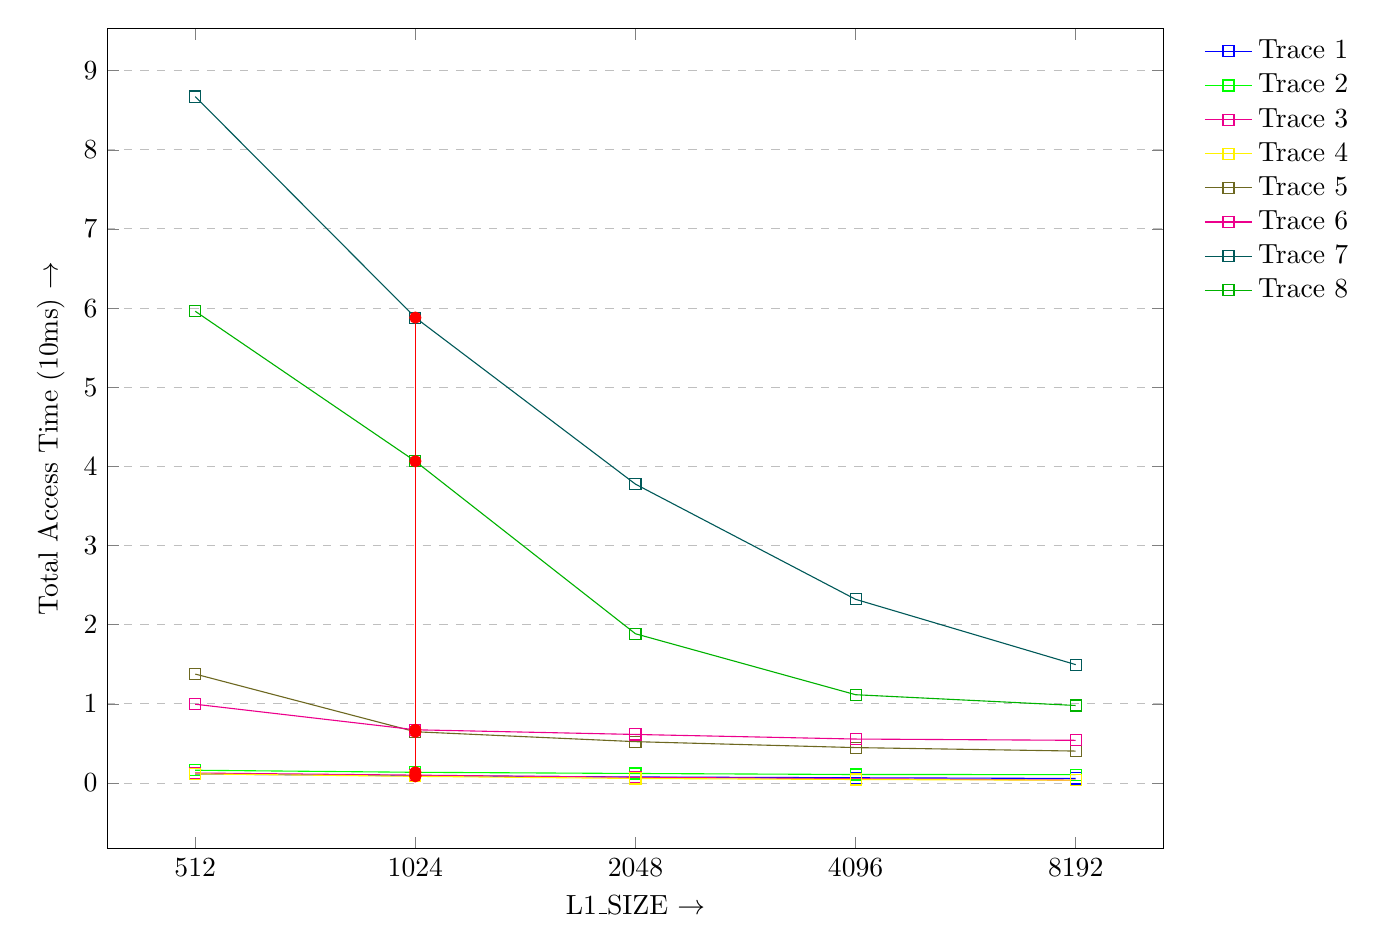
\begin{tikzpicture}
    \begin{axis}[
        xlabel={L1\_SIZE $\rightarrow$},
        ylabel={Total Access Time (10ms) $\rightarrow$},
        xtick=data,
        symbolic x coords={512,1024,2048,4096,8192},
        legend pos=outer north east,
        legend style={draw=none},
        ymajorgrids=true,
        grid style=dashed,
    ]
    \addplot[color=blue,mark=square] coordinates {
        (512,0.115) (1024,0.092) (2048,0.077) (4096,0.067) (8192,0.058)};
    \addplot[color=green,mark=square] coordinates {
        (512,0.162) (1024,0.136) (2048,0.121) (4096,0.108) (8192,0.107)};
    \addplot[color=magenta,mark=square] coordinates {
        (512,0.127) (1024,0.1) (2048,0.073) (4096,0.055) (8192,0.037)};
    \addplot[color=yellow,mark=square] coordinates {
        (512,0.116) (1024,0.085) (2048,0.058) (4096,0.045) (8192,0.036)};
    \addplot[color=olive!70!black,mark=square] coordinates {
        (512,1.377) (1024,0.648) (2048,0.523) (4096,0.448) (8192,0.404)};
    \addplot[color=magenta,mark=square] coordinates {
        (512,0.996) (1024,0.673) (2048,0.614) (4096,0.556) (8192,0.54)};
    \addplot[color=teal!70!black,mark=square] coordinates {
        (512,8.672) (1024,5.88) (2048,3.776) (4096,2.321) (8192,1.496)};
    \addplot[color=green!70!black,mark=square] coordinates {
        (512,5.96) (1024,4.065) (2048,1.886) (4096,1.116) (8192,0.98)};
    \addplot[color=red,mark=*] coordinates {
        (1024,0.092) (1024,0.136) (1024,0.1) (1024,0.085) (1024,0.648) (1024,0.673) (1024,5.88) (1024,4.065)};
    \legend{Trace 1,Trace 2,Trace 3,Trace 4,Trace 5,Trace 6,Trace 7,Trace 8,}
    \end{axis}
    \end{tikzpicture}
    \caption{Variation in L1 size}\label{fig:L1}
    \end{figure}


\begin{itemize}
    \item \textbf{Theoretical Expectation} : As the L1 cache size increases, the cache can store more blocks, which reduces the number of cache misses. Therefore, we expect to see a \textcolor{blue}{decrease in the miss rate and total access time as the L1 cache size increases.}  However, increasing the L1 cache size also increases the access latency, which may offset the reduction in the miss rate. Hence, there is an optimal L1 cache size that minimizes the total access time.
    \item We can see that for all the traces, the total access time decreases as the L1 size increases which matches with theoretical expectation. The variation is significant for trace 5, trace 7 and trace 8. 
\end{itemize}

\newpage
\subsubsection{Variation in L1 Associativity}
In the third graph, vary the third parameter L1 associativity between 1, 2, 4, 8, 16, and
keep block size, L1 size, L2 size and L2 associativity fixed at 64, 1024, 65536, 8.
\begin{figure}[h]
    \centering
    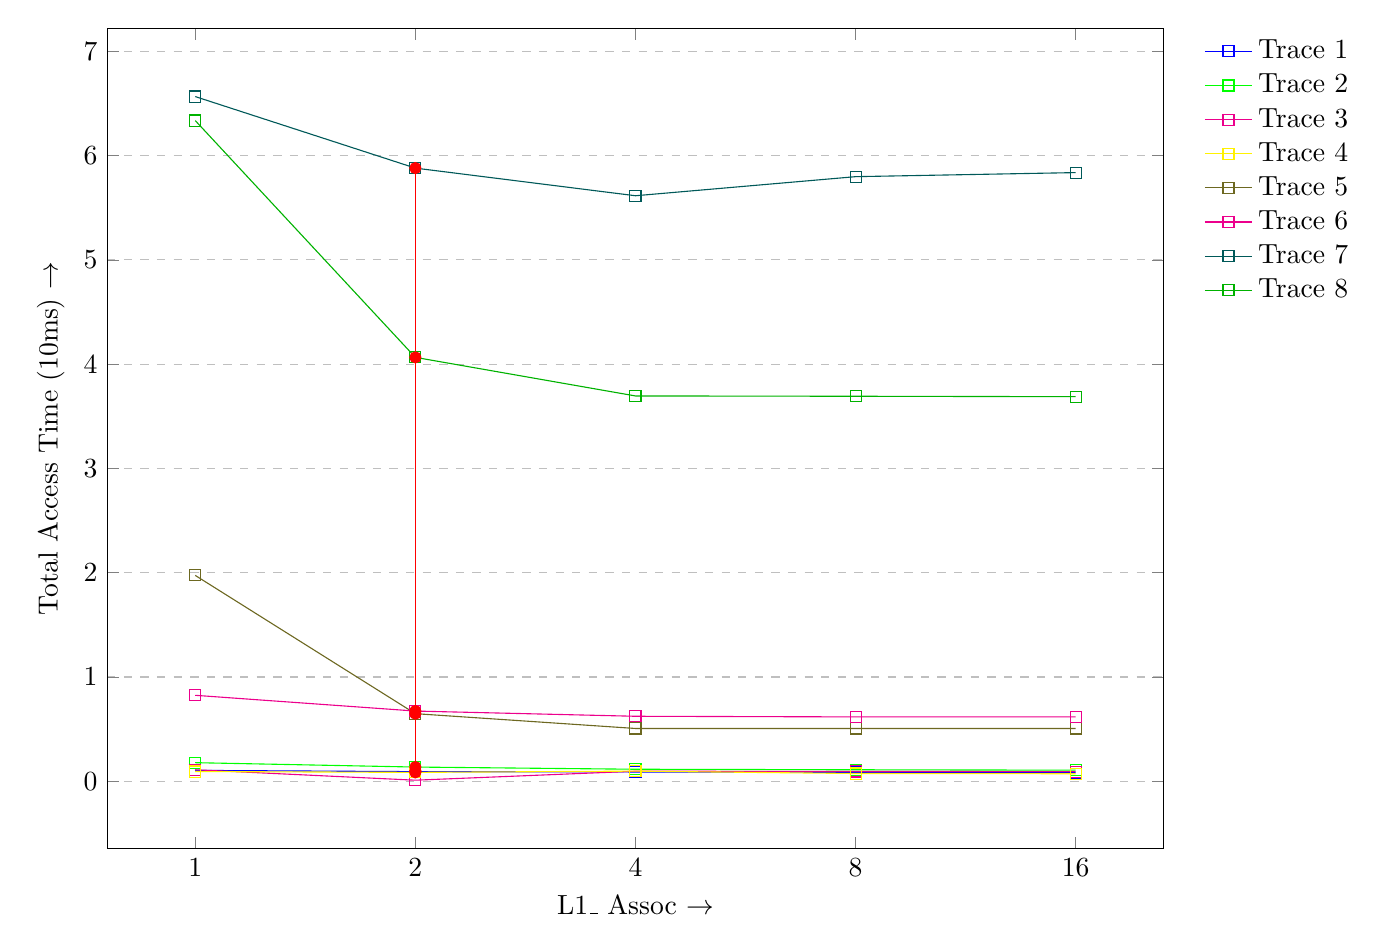
\begin{tikzpicture}
    \begin{axis}[
        xlabel={L1\_ Assoc $\rightarrow$},
        ylabel={Total Access Time (10ms) $\rightarrow$},
        xtick=data,
        symbolic x coords={1,2,4,8,16},
        legend pos=outer north east,
        legend style={draw=none},
        ymajorgrids=true,
        grid style=dashed,
    ]
    \addplot[color=blue,mark=square] coordinates {
        (1,0.104) (2,0.092) (4,0.089) (8,0.086) (16,0.084)};
    \addplot[color=green,mark=square] coordinates {
        (1,0.178) (2,0.136) (4,0.115) (8,0.11) (16,0.106)};
    \addplot[color=magenta,mark=square] coordinates {
        (1,0.11) (2,0.01) (4,0.096) (8,0.094) (16,0.092)};
    \addplot[color=yellow,mark=square] coordinates {
        (1,0.093) (2,0.085) (4,0.097) (8,0.074) (16,0.072)};
    \addplot[color=olive!70!black,mark=square] coordinates {
        (1,1.974) (2,0.648) (4,0.506) (8,0.506) (16,0.506)};
    \addplot[color=magenta,mark=square] coordinates {
        (1,0.824) (2,0.673) (4,0.623) (8,0.617) (16,0.617)};
    \addplot[color=teal!70!black,mark=square] coordinates {
        (1,6.566) (2,5.88) (4,5.615) (8,5.798) (16,5.837)};
    \addplot[color=green!70!black,mark=square] coordinates {
        (1,6.336) (2,4.065) (4,3.695) (8,3.692) (16,3.688)};
    \addplot[color=red,mark=*] coordinates {
        (2,0.092) (2,0.136) (2,0.1) (2,0.085) (2,0.648) (2,0.673) (2,5.88) (2,4.065)};
    \legend{Trace 1,Trace 2,Trace 3,Trace 4,Trace 5,Trace 6,Trace 7,Trace 8,}
    \end{axis}
    \end{tikzpicture}
    \caption{Variation in L1 Associativity}\label{fig:L1A}
    \end{figure}



\begin{itemize}
    \item  \textbf{Theoretical Expectation} : As the L1 cache associativity increases, the cache can store more blocks and hence reduce the number of cache misses. Therefore, we expect to see a \textcolor{blue}{ decrease in the miss rate and total access time as the L1 associativity increases }. However, increasing the associativity also increases the access latency, which may \textcolor{red}{ offset the reduction in the miss rate.} Hence, there is an optimal L1 associativity that minimizes the total access time.
    \item From the Graph we can conclude that the access time decreases as the associativity increases then increases at higher values for some traces which matches with Theoretical Expectation. The effect is significant for trace 7 and trace 8. The default value of associativity is 2 which is the optimal value for some of the traces.
\end{itemize}


\newpage
\subsubsection{Variation in L2 Size}
In the fourth graph, vary the fourth parameter L2 size between 16384, 32768, 65536,
131072, 262144, and keep block size, L1 size, L1 associativity and L2 associativity fixed
at 64, 1024, 2, 8.

\begin{figure}[h]
    \centering
    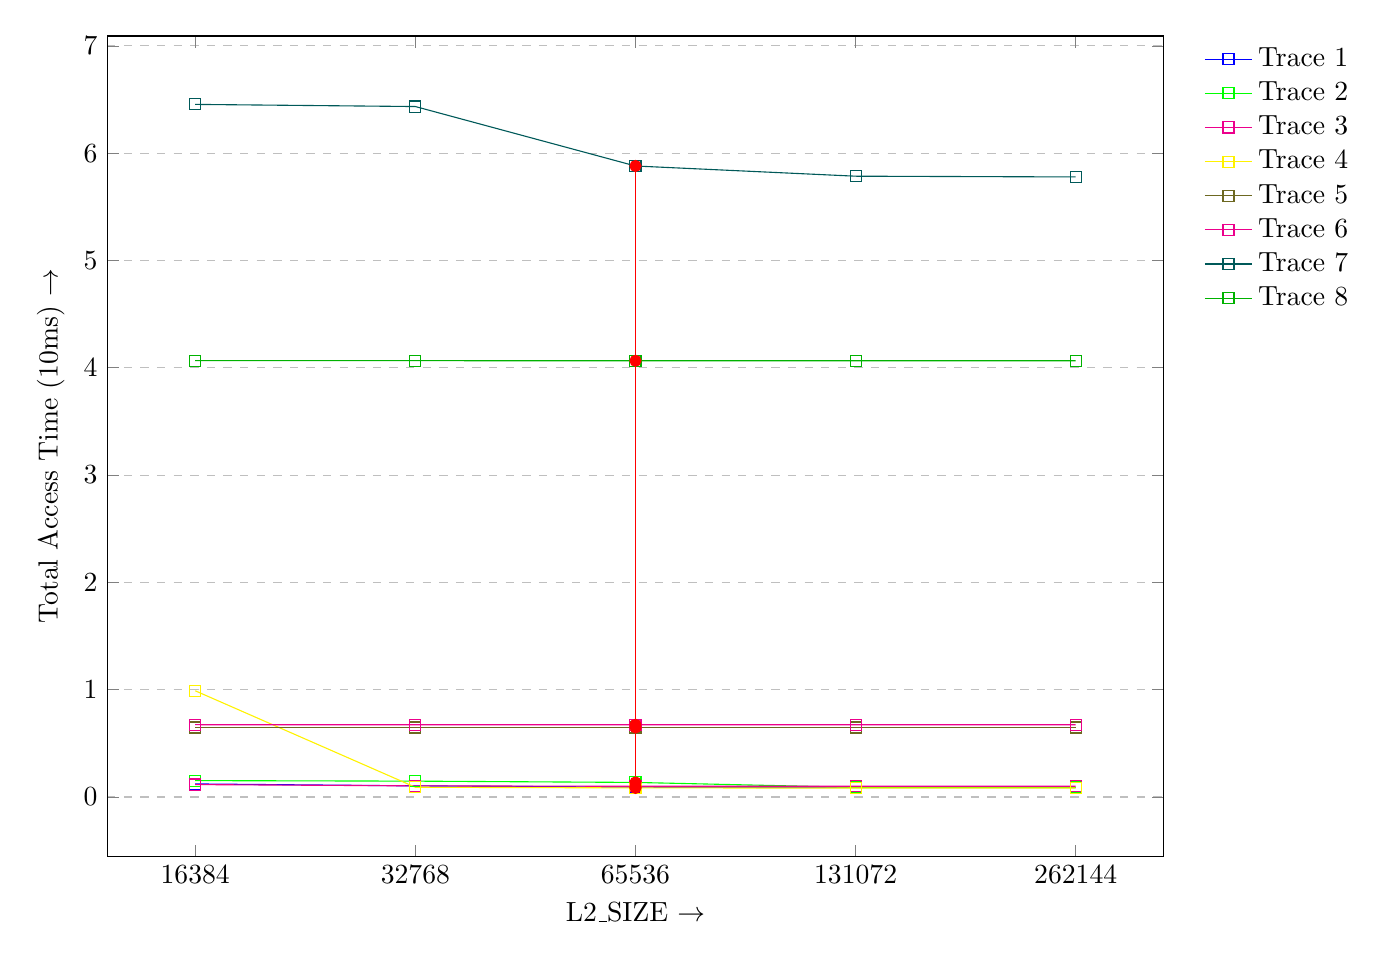
\begin{tikzpicture}
    \begin{axis}[
        xlabel={L2\_SIZE $\rightarrow$},
        ylabel={Total Access Time (10ms) $\rightarrow$},
        xtick=data,
        symbolic x coords={16384,32768,65536,131072,262144},
        legend pos=outer north east,
        legend style={draw=none},
        ymajorgrids=true,
        grid style=dashed,
    ]
    \addplot[color=blue,mark=square] coordinates {
        (16384,0.122) (32768,0.104) (65536,0.092) (131072,0.087) (262144,0.087)};
    \addplot[color=green,mark=square] coordinates {
        (16384,0.153) (32768,0.148) (65536,0.136) (131072,0.09) (262144,0.09)};
    \addplot[color=magenta,mark=square] coordinates {
        (16384,0.116) (32768,0.104) (65536,0.1) (131072,0.1) (262144,0.1)};
    \addplot[color=yellow,mark=square] coordinates {
        (16384,0.99) (32768,0.091) (65536,0.085) (131072,0.084) (262144,0.084)};
    \addplot[color=olive!70!black,mark=square] coordinates {
        (16384,0.648) (32768,0.648) (65536,0.648) (131072,0.648) (262144,0.648)};
    \addplot[color=magenta,mark=square] coordinates {
        (16384,0.674) (32768,0.673) (65536,0.673) (131072,0.673) (262144,0.673)};
    \addplot[color=teal!70!black,mark=square] coordinates {
        (16384,6.454) (32768,6.434) (65536,5.88) (131072,5.785) (262144,5.778)};
    \addplot[color=green!70!black,mark=square] coordinates {
        (16384,4.066) (32768,4.066) (65536,4.065) (131072,4.065) (262144,4.065)};
    \addplot[color=red,mark=*] coordinates {
        (65536,0.092) (65536,0.136) (65536,0.1) (65536,0.085) (65536,0.648) (65536,0.673) (65536,5.88) (65536,4.065)};
    \legend{Trace 1,Trace 2,Trace 3,Trace 4,Trace 5,Trace 6,Trace 7,Trace 8,}
    \end{axis}
    \end{tikzpicture}
    \caption{Variation in L2 Size}\label{fig:L2}
    \end{figure}

\begin{itemize}
    \item \textbf{Theoretical Expectation} : As the L2 cache size increases, the cache can store more blocks and hence reduce the number of cache misses. Therefore,\textcolor{blue}{ we expect to see a decrease in the miss rate and total access time as the L2 cache size increases.} However, increasing the L2 cache size also increases the access latency, which may offset the reduction in the miss rate. Hence, there is an optimal L2 cache size that minimizes the total access time.
    \item From the Graph we can conclude that the access time decreases negligibly for most traces as the L2 size increases and significantly for trace 7  which matches theoretical expectation. This means that the L2 size is not a major factor in determining the access time and affects significatly only if L1 miss rate is high for a trace. The default value of L2 size is 65536.
\end{itemize}


\newpage
\subsubsection{Variation in L2 Associativity}
In the fifth graph, vary the fifth parameter L2 associativity between 1, 2, 4, 8, 16, and
keep block size, L1 size, L1 associativity and L2 size fixed at 64, 1024, 2, 65536.
\begin{figure}[h]
    \centering
    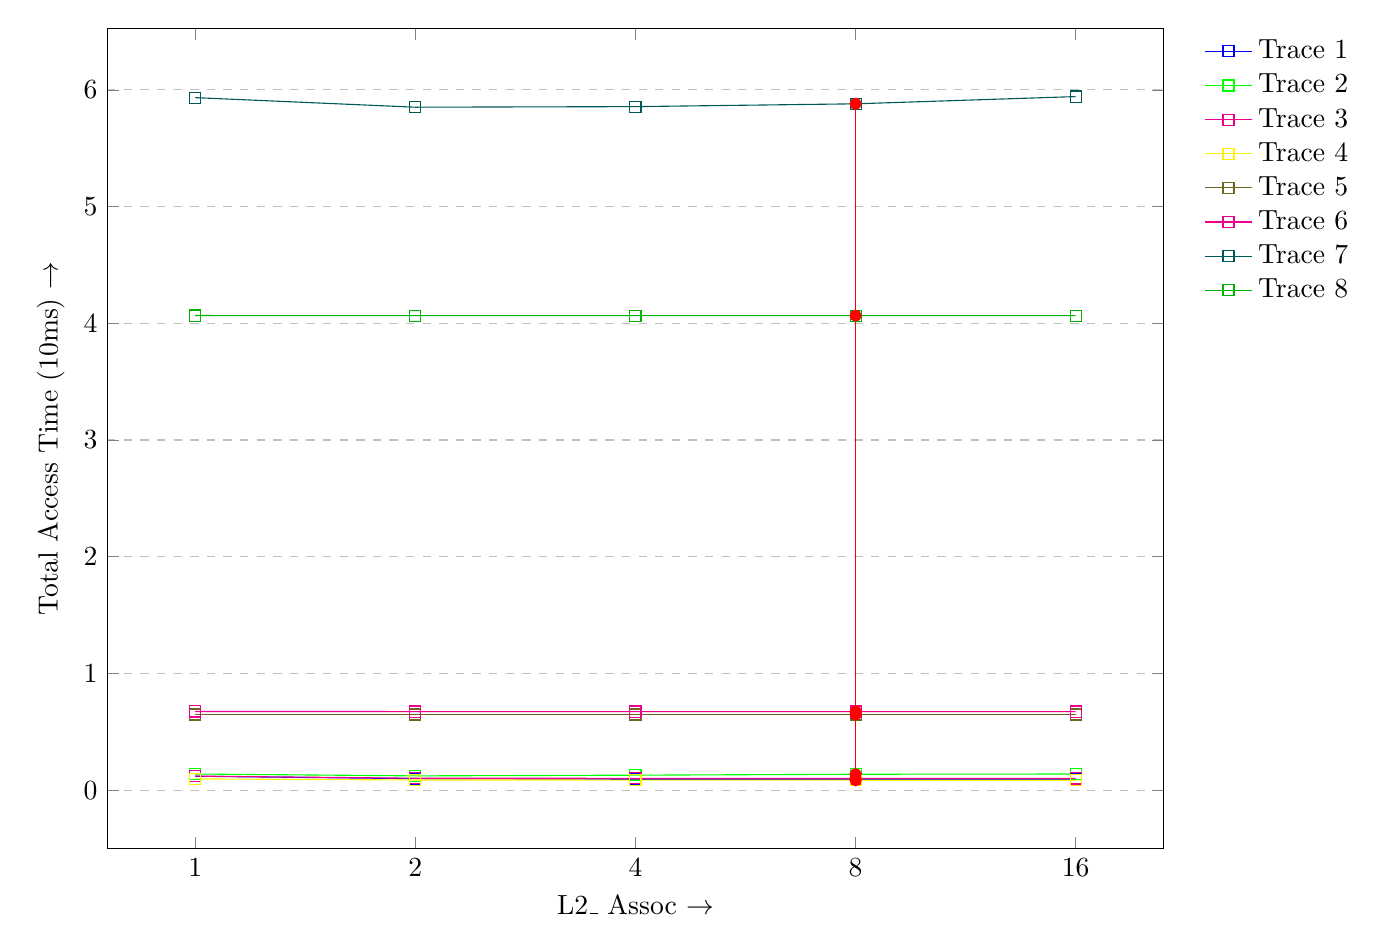
\begin{tikzpicture}
    \begin{axis}[
        xlabel={L2\_ Assoc $\rightarrow$},
        ylabel={Total Access Time (10ms) $\rightarrow$},
        xtick=data,
        symbolic x coords={1,2,4,8,16},
        legend pos=outer north east,
        legend style={draw=none},
        ymajorgrids=true,
        grid style=dashed,
    ]
    \addplot[color=blue,mark=square] coordinates {
        (1,0.119) (2,0.098) (4,0.093) (8,0.092) (16,0.092)};
    \addplot[color=green,mark=square] coordinates {
        (1,0.138) (2,0.122) (4,0.128) (8,0.136) (16,0.138)};
    \addplot[color=magenta,mark=square] coordinates {
        (1,0.12) (2,0.102) (4,0.101) (8,0.1) (16,0.1)};
    \addplot[color=yellow,mark=square] coordinates {
        (1,0.096) (2,0.087) (4,0.086) (8,0.085) (16,0.085)};
    \addplot[color=olive!70!black,mark=square] coordinates {
        (1,0.648) (2,0.648) (4,0.648) (8,0.648) (16,0.648)};
    \addplot[color=magenta,mark=square] coordinates {
        (1,0.674) (2,0.673) (4,0.673) (8,0.673) (16,0.673)};
    \addplot[color=teal!70!black,mark=square] coordinates {
        (1,5.933) (2,5.851) (4,5.856) (8,5.88) (16,5.942)};
    \addplot[color=green!70!black,mark=square] coordinates {
        (1,4.066) (2,4.065) (4,4.065) (8,4.065) (16,4.065)};
    \addplot[color=red,mark=*] coordinates {
        (8,0.092) (8,0.136) (8,0.1) (8,0.085) (8,0.648) (8,0.673) (8,5.88) (8,4.065)};
    \legend{Trace 1,Trace 2,Trace 3,Trace 4,Trace 5,Trace 6,Trace 7,Trace 8,}
    \end{axis}
    \end{tikzpicture}
    \caption{Variation in L2 Associativity}\label{fig:L2A}
    \end{figure}


\begin{itemize}
    \item  \textbf{Theoretical Expectation} : As the L2 cache associativity increases, the cache can store more blocks and hence reduce the number of cache misses. Therefore, we expect to see a \textcolor{blue}{ decrease in the miss rate and total access time as the L2 associativity increases.} However, increasing the associativity also increases the access latency, which may \textcolor{red}{ offset the reduction in the miss rate.} Hence, there is an optimal L2 associativity that minimizes the total access time.
    \item From the Graph we can see that the access time remains constant for most traces except trace 7 for which it decreases slightly then increases slightly which matches theoretical expectation.This means that the L2 associativity is not a major factor in determining the access time and affects significatly only if L1 miss rate is high for a trace. The default value of L2 associativity is 8.
\end{itemize}

\newpage

\section{Instructions to run the code}

run the following command in the terminal

\begin{lstlisting}[backgroundcolor = \color{light-gray},
    language = bash,
    xleftmargin = 0cm,
    framexleftmargin = 1em]
    $ make run
\end{lstlisting}

You can adjust the parameters in the Makefile to run the code for different traces and different cache parameters.
\begin{lstlisting}[backgroundcolor = \color{light-gray},
    language = python,
    xleftmargin = 0cm,
    framexleftmargin = 1em]
    @./cache_simulate 64 1024 2 65536 8 memory_trace_files/trace1.txt
\end{lstlisting}
Here the parameters are in the order of block size, L1 size, L1 associativity, L2 size, L2 associativity and the trace file name.


\section{Work Split}
\begin{table}[h]
    \centering
    \begin{tabular}{|c|c|c|}
    \hline
    \textbf{S.No.} & \textbf{Team member} & \textbf{\%Work Split} \\ \hline
    1              & Dhruv Gupta          & 50\%                  \\ \hline
    2              & Niranjan Sarode      & 50\%                  \\ \hline
    \end{tabular}
    \caption{Token Distribution}
    \label{tab:token-split}
    \end{table}

\end{document}